\documentclass[a4paper,10pt]{article}

\usepackage[utf8]{inputenc}
%\usepackage[T1]{fontenc}

\usepackage{textcomp}           % Extra Symbole (Grad Celsius etc.)
\usepackage{amssymb,amsmath}    % Schöne Formeln (AMS = American Mathematical Society)
\usepackage{graphicx}           % Bilder und Seitenränder
\usepackage{subcaption}			% captions for subfigures
\usepackage{booktabs}           % Schönere Tabellen
\usepackage{colortbl}           % Farbige Tabellen

%\usepackage{tcolorbox}			% schöne bunte Boxen
\usepackage{mathtools}			% \mathclap für ordentliche \underbrace-			environments
\usepackage[left=2cm,right=2cm,top=2cm,bottom=2cm]{geometry}			% Pagelayout mit \newgeometry, \restoregeometry
\usepackage{float}
\usepackage{wrapfig}
\usepackage{enumitem}
\usepackage{float}
\usepackage{braket}
\usepackage{caption}
\usepackage{verbatim}
\usepackage[per-mode=reciprocal,output-decimal-marker={.},binary-units=true,separate-uncertainty=true]{siunitx}
\usepackage[breaklinks=true,colorlinks=true,linkcolor=blue,urlcolor=blue,citecolor=blue]{hyperref}
\usepackage{physics}
\usepackage{url}
\usepackage{subcaption}
\usepackage{calrsfs}
\usepackage{tikz}
\usetikzlibrary{decorations, positioning, intersections, calc, shapes,arrows, scopes}
\DeclareMathAlphabet{\pazocal}{OMS}{zplm}{m}{n}

\graphicspath{{./img/}}

\newcommand{\dif}{\mathrm{d}}

\bibliographystyle{instant}

\renewcommand{\k}{\mathbf{k}}
\begin{document}
\begin{titlepage}
 \begin{center}
 \Large{Lab Course in Experimental Physics: Optics}
 \end{center}
 \begin{center}
  \LARGE{\textbf{Focus locking of a tunable lens for optical transportation of ultracold atoms}}
 \end{center}
 \begin{center}
 \large Marco \textsc{Canteri} \\
 marco.canteri@student.uibk.ac.at\\
 \end{center}

 \begin{center}
 \vspace{1cm}
 Innsbruck, \today
 \vspace{1cm}
 \end{center}

 \begin{abstract}
In this project a setup for optical transportation of ultracold atoms has been realized. The focus of a laser was shifted with a tunable optotune lens controlled by custom electronics, and locked with a feedback signal generated from a quadrant photodiode.
\end{abstract}
  \vspace{1cm}

 \begin{center}
 
\includegraphics[scale=0.567]{img/uibk}
 \end{center}

\end{titlepage}

\section{Introduction}

\section{Theoretical background}
\subsection{Focus tunable lens}
\subsection{Cylindrical lens}

\section{Experiment setup}
The setup prepared can be divided in two parts, the optical setup and the electronics part used to control the optics. The main idea of the experiment is to control and lock the focus of a 1064nm laser. This is done with an optotune EL-16-40-TC focus tunable lens \cite{lens_datasheet}. To lock the focus, a part of the beam has been send through a cylindrical lens, and then measured with a quadrant photodiode. The cylindrical lens deforms the spherical symmetry of the beam such that when projected on the photodiode, the light will not hit all the four quadrants uniformly. The signal generated from the quadrants can be used as a measure of relative focus, therefore we can feedback this signal to the lens and get focus locking.
\subsection{Optical setup}
\begin{figure}
\centering
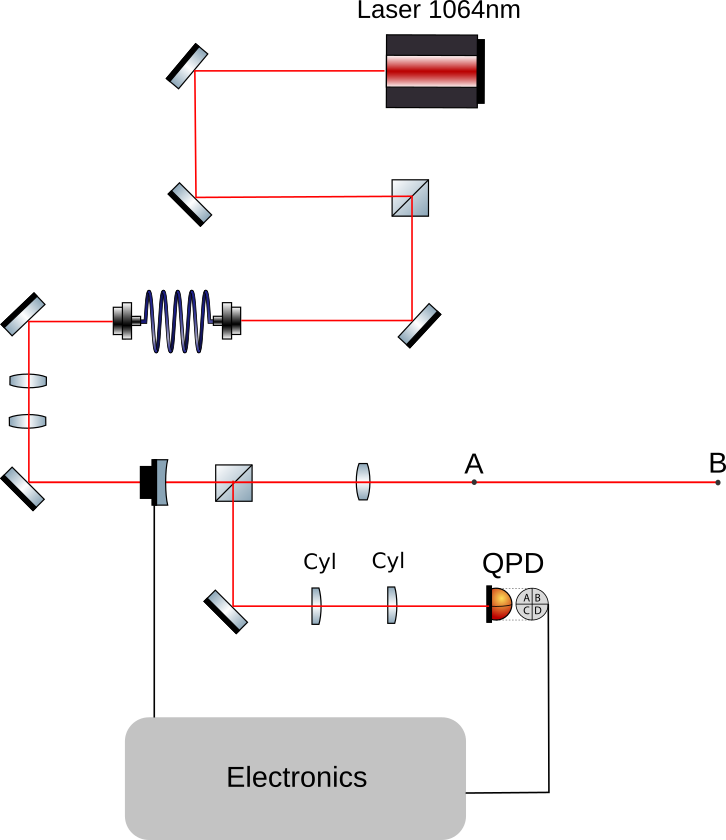
\includegraphics[width = .5\textwidth]{opticsetup}
\caption{Optical setup, after the fiber a 1064nm laser light is collimated and sent trough a tunable lens. Two cylindrical lens and a quadrant photodiode are used to generate an error signal for the focus which is feedback to the lens with some electronics. The focus of the laser could be changed from point A to point B, roughly 80 cm.} \label{img:opticsetup}
\end{figure}
The setup is depicted in figure \ref{img:opticsetup}. We used a 1064nm laser, the light is split with a beam splitter, one beam is used in another experiment, while the beam showed in the setup is coupled with a fiber in order to filter the modes and have at the end a pure Gaussian beam. After the fiber the beam is expanded with two lenses to roughly 10 mm diameter. Subsequently, the beam pass through a tunable lens controlled by the electronic part. The lens can change focus from  -500 to +333 mm, but in this experiment we kept the focus negative. A beam splitter is used to create a beam for measuring the focus shift, while the transmitted beam is focused with a 400mm lens between point A and B depending on the current applied to the lens. The trick of using a tunable and a convergent lens instead of simply the optotune lens is to keep the waist of the beam constant, in fact a non constant beam would change trapping frequency and trap depth resulting in losing atom during the transportation \cite{opticaltransportation}


\subsection{Electronic PID}

\section{Conclusion}

 \begin{thebibliography}{99}
\bibitem{lens_datasheet}
 \textsc{Optotune}, \textit{EL-16-40-TC}, \url{https://www.optotune.com/images/products/Optotune%20EL-16-40-TC.pdf}
%
 \bibitem{opticaltransportation}
 \textsc{J. Léonard, M Lee, A. Morales, T. Karg, T Esslinger, T. Donner}, \textit{Optical transport and manipulation of an ultracold atomic cloud using focus-tunable lenses}, New Journal of Physics, volume 16 number 9, 2014

%
% \bibitem{bergmann}
% \textsc{Bergmann-Schäfer}, \textit{Gase, Nanosysteme, Flüssigkeiten}, \textit{Band 5} (de Gruyter, 2005)
%
% \bibitem{cold_cathode}
% \textsc{LDS Vacuum Shopper}, \textit{Cold Cathode Gauges}, \url{http://www.ldsvacuumshopper.com/cocaga.html}
%
% \bibitem{script}
% \textsc{Jennifer Meyer, Roland Wester}, \textit{Versuch im Fortgeschrittenen Praktikum FP3: Supersonische Düsenstrahlen}
%
% \bibitem{lifetime}
% \textsc{Cullen P.J., Milosavljevic V.} (2015) Prog. Theor. Exp. Phys.2015/6, 063J01 . doi:10.1093/ptep/ptv070
%
% \bibitem{illinois}
% \textsc{McCall research group}, \textit{Supersonic Expansion Discharge Source}, \url{http://bjm.scs.illinois.edu/past/source.php}
 \end{thebibliography}
\end{document}
